\documentclass[tikz,border=6pt]{standalone}
\usepackage[T1]{fontenc}
\usepackage[utf8]{inputenc}
\usepackage[scaled=.92]{helvet}
\usetikzlibrary{arrows.meta,positioning,calc,backgrounds}

\definecolor{navy}{HTML}{163B65}
\definecolor{bluefill}{HTML}{E4EDF8}
\definecolor{greenfill}{HTML}{E3F2EC}
\definecolor{textgray}{HTML}{4A5563}
\definecolor{accent}{HTML}{B4541A}

\begin{document}
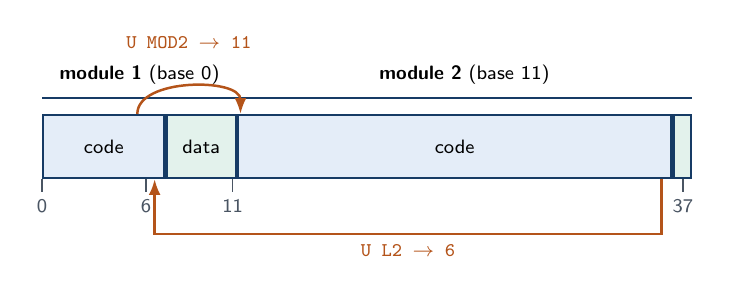
\begin{tikzpicture}[
  font=\sffamily\scriptsize, >=Latex,
  seg/.style={draw=navy, line width=0.8pt, minimum height=8mm, inner sep=0pt, align=center},
  ref/.style={-{Latex[length=2mm]}, line width=0.9pt, draw=accent}
]
% scale: 1 word = 2.2 mm  (module 1 = 11 words, module 2 = 26 words)
\def\u{2.2mm}
\node[seg, fill=bluefill,  minimum width=7*\u,  anchor=south west] (c1) at (0,0) {code};
\node[seg, fill=greenfill, minimum width=4*\u,  anchor=south west] (d1) at (c1.south east) {data};
\node[seg, fill=bluefill,  minimum width=25*\u, anchor=south west] (c2) at (d1.south east) {code};
\node[seg, fill=greenfill, minimum width=1*\u,  anchor=south west] (d2) at (c2.south east) {};

% module labels
\draw[navy, line width=0.6pt] ($(c1.north west)+(0,2mm)$) -- node[above=0.5mm, text=black] {\textbf{module 1} (base 0)} ($(d1.north east)+(0,2mm)$);
\draw[navy, line width=0.6pt] ($(c2.north west)+(0,2mm)$) -- node[above=0.5mm, text=black] {\textbf{module 2} (base 11)} ($(d2.north east)+(0,2mm)$);

% addresses
\foreach \a/\x in {0/0, 6/6, 11/11, 37/37} {
  \draw[textgray] ($(c1.south west)+(\x*\u,0)$) -- ++(0,-1.6mm);
  \node[below=1.4mm, text=textgray] at ($(c1.south west)+(\x*\u,0)$) {\a};
}

% resolved external references
\draw[ref] ($(c1.north west)+(5.5*\u,0)$) to[out=90,in=90,looseness=0.9] node[above, text=accent, pos=0.5, yshift=3.5mm] {\ttfamily U MOD2 $\rightarrow$ 11} ($(c2.north west)+(0.2*\u,0)$);
\draw[ref] ($(c2.south west)+(24.5*\u,0)$) -- ++(0,-7mm) -| node[below, text=accent, pos=0.25] {\ttfamily U L2 $\rightarrow$ 6} ($(c1.south west)+(6.5*\u,0)$);
\end{tikzpicture}
\end{document}
